\newcommand{\ZZ}{\ensuremath{\mathbb Z}}

% \newcounter{saveenumi}
% \newcommand{\seti}{\setcounter{saveenumi}{\value{enumi}}}
% \newcommand{\conti}{\setcounter{enumi}{\value{saveenumi}}}

\paragraph{Problemas num\'ericos}
Como todas las ciencias, la matem\'atica est\'a basada en la experiencia.
En los pr\'oximos d\'{\i}as, exploraremos un sistema matem\'atico que
todas las personas han experimentado, el sistema de los n\'umeros enteros.
Los n\'umeros enteros son:
\begin{displaymath}
	\dots,\,-3,\,-2,\,-1,\,0,\,1,\,2,\,3,\,\dots
\end{displaymath}
%
Para referirnos al conjunto de n\'umeros enteros usamos el s\'{\i}mbolo
$\ZZ$. O sea,
\begin{math}
	\mathbb Z=\{\dots,\,-3,\,-2,\,-1,\,0,\,1,\,2,\,3,\,\dots\}
\end{math}.

Como sabemos, es posible sumar y multiplicar en $\ZZ$.
Tambi\'en es posible restar en $\ZZ$.
Sin embargo, no siempre es posible dividir.
Por ejemplo, si intent\'asemos dividir $1$ entre $2$, buscar\'{\i}amos
un entero $x\in\ZZ$ tal que $2x=1$ !`Pero no existe tal entero!

En la escuela, aprendemos a dividir con resto. El proceso se conoce
como el \emph{algoritmo de divisi\'on}. Por ejemplo, si dividimos
$1068$ entre $7$, obtenemos el cociente $152$ y resto $4$:
\begin{displaymath}
	1068\,=\,7\cdot 152\,+\,4
	\text{ .}
\end{displaymath}
%
En general, si $m$ es un entero positivo, entonces podemos aplicar este
proceso para dividir cualquier otro entero $a$ por $m$, obteniendo un
resto, $q$, y un resto, $r$, de manera que $r$ sea uno de los n\'umeros
$0,\,1,\,2,\,\dots,\,m-1$. Podemos resumir esto de la siguiente manera:
$a=m\cdot q+r$ y $0\leq r<m$.

A pesar de la simplicidad del algoritmo de divisi\'on, sus consecuencias
pueden ser inesperadamente profundas y es un proceso que se puede
generalizar de diversas maneras. Una de las aplicaciones b\'asicas
del algoritmo de divisi\'on se relaciona con c\'omo escribimos los
n\'umeros. Lo m\'as usual es usar la notaci\'on \emph{en base $10$},
el \emph{sistema decimal}. Por ejemplo, $1068$ es s\'olo una forma de
escribir $1\cdot 10^3+0\cdot 10^2+6\cdot 10+8$. Pero podr\'{\i}amos
utilizar otra base, en lugar de base $10$.
Veamos c\'omo escribir $1068$ \emph{en base $7$}.
Empezamos usando el algoritmo de divisi\'on para dividir $1068$ entre $7$.
Ya hemos hecho esto m\'as arriba y el resultado fue $1068=7\cdot 152+4$.
A continuaci\'on dividimos el cociente anterior, $152$, entre $7$,
obteniendo un nuevo cociente, $21$, y un nuevo resto, $5$, es decir,
$152=7\cdot 21+5$. Si seguimos este procedimiento, encontramos las
siguientes ecuaciones:
\begin{displaymath}
	\begin{aligned}
		1068 & \,=\,7\cdot 152\,+\,4
			\text{ ,} \\
		152 & \,=\,7\cdot 21\,+\,5
			\text{ ,} \\
		21 & \,=\,7\cdot 3\,+\,0
			\text{ ,} \\
		3 & \,=\,7\cdot 0\,+\, 3
			\text{ .}
	\end{aligned}
	%
\end{displaymath}
%
A partir de estas igualdades, podemos concluir que
\begin{displaymath}
	1068\,=\,3\cdot 7^3\,+\,0\cdot 7^2\,+\,5\cdot 7\,+\,4
	\text{ .}
\end{displaymath}
%
De esta manera, el n\'umero que en base diez se escribe
$1068$ es igual al n\'umero que en base siete se escribe
$(3054)_7$. Los cuatro ``d\'{\i}gitos'' en la escritura en base siete
son los cuatro restos que aparecieron en las cuatro ecuaciones anteriores.

\begin{enumerate}[label=P\arabic*]
	\item\label{item:cambiar}
		Si $N=32701$ (en base diez), escribir $N$ en base dos,
		en base tres y en base once. En este \'ultimo caso,
		hay que introducir un nuevo ``d\'{\i}gito'', $A=10$.
	\item\label{item:operar}
		Sin cambiar la base,
		\begin{enumerate}[label=(\alph*)]
			\item\label{item:operar:sumar}
				sumar $(6153)_7$ con $(3455)_7$,
			\item\label{item:operar:restar}
				restar $(2346)_7$ a $(4354)_7$,
			\item\label{item:operar:multiplicar}
				multiplicar $(632)_7$ por $(435)_7$,
			\item\label{item:operar:dividir}
				dividir $(5602)_7$ por $(43)_7$.
		\end{enumerate}
		%
	\seti
\end{enumerate}
%

\paragraph{Exploraci\'on}
Para poder entender mejor $\ZZ$, tambi\'en investigaremos otros sistemas
alternativos. Algunos ejemplos de estos sistemas aritm\'eticos son los
\emph{enteros modulares} y su \emph{aritm\'etica modular}. Para explicar
lo que esto significa, veamos un ejemplo.

Escribamos $\ZZ_7$ para referirnos al conjunto $\{0,1,2,3,4,5,6\}$.
El conjunto $\ZZ_7$ es igual al conjunto de posibles restos de dividir por
$7$ cuando aplicamos el algoritmo de divisi\'on. En este sistema,
el n\'umero $7$ es el \emph{m\'odulo} del sistema y $\ZZ_7$ es el
\emph{sistema de residuos m\'odulo $7$}. Vamos a dar a $\ZZ_7$
dos operaciones: una suma y una multiplicaci\'on. Para describir estas
operaciones, disponemos los elementos de $\ZZ_7$ en un c\'{\i}rculo
de la siguiente manera:

\begin{displaymath}
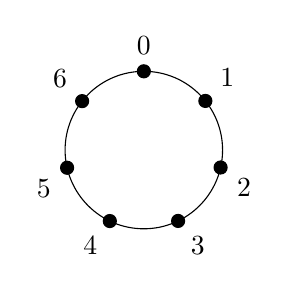
\begin{tikzpicture}
	\draw (0,0) circle[radius=1];
	\node[draw, circle, scale=.5, fill=black, label=above:\(0\)] (0) at (90:1) {};
	\foreach \i [remember=\i as \j (initally 0)] in {1,...,6} {
		\node[draw, circle, scale=.5, fill=black, label=90-51.4*\i:\(\i\)] (\i) at (90-51.4*\i:1) {};
	}
\end{tikzpicture}
%
\end{displaymath}
%

Supongamos que queremos sumar dos elementos de $\ZZ_7$, por ejemplo,
$5$ y $6$. Entonces, empezamos con $6$ y nos movemos en sentido horario
$5$ unidades. Como terminamos en el n\'umero $4$, podemos decir que
$5+6=4$ en $\ZZ_7$. Los siguientes son otros ejemplos de la suma
en $\ZZ_7$:
\begin{displaymath}
	1+2\,=\,3
	\text{ ;}\quad
	6+6\,=\,5
	\text{ ;}\quad
	2+5\,=\,0
	\text{ ;}\quad
	3+4+5+6\,=\,4
	\text{ .}
\end{displaymath}
%
Tambi\'en podemos multiplicar en $\ZZ_7$. Si queremos multiplicar
$6$ con $2$ en $\ZZ_7$, simplemente sumamos $6$ consigo mismo dos veces,
pero en $\ZZ_7$: $6\cdot 2=6+6=5$. De la misma manera, para multiplicar $5$
por $4$, sumamos $5$ consigo cuatro veces:
$5\cdot 4=5+5+5+5=6$. Los siguientes son otros ejemplos de la
multiplicaci\'on en $\ZZ_7$:
\begin{displaymath}
	2\cdot 3\,=\,6
	\text{ ;}\quad
	3\cdot 4\,=\,5
	\text{ ;}\quad
	4\cdot 6\,=\,3
	\text{ ;}\quad
	5\cdot 5\cdot 5\,=\,6
	\text{ .}
\end{displaymath}
%

Habiendo entendido la suma y la multiplicaci\'on podemos intentar
realizar otro tipo de operaciones en $\ZZ_7$.

\begin{enumerate}[label=P\arabic*]
	\conti
	\item\label{item:otras-operaciones}
		?`Cu\'ales de las siguientes operacioraciones se pueden
		realizar en $\ZZ_7$?
		\begin{displaymath}
			4\cdot 5
			\text{ ,}\quad
			2-6
			\text{ ,}\quad
			1/2
			\text{ ,}\quad
			2/5
			\text{ ,}\quad
			\sqrt 2
			\text{ ,}\quad
			\sqrt{-3}
			\text{ ,}\quad
			\sqrt{-1}
			\text{ ,}\quad
			\sqrt[3] 6
			\text{ .}
		\end{displaymath}
		%
		Por ejemplo, en el tercer caso, $1/2$, empezamos
		respondiendo qu\'e significa la expresi\'on ``$1/2$''.
		La expresi\'on ``$1/2$'' es un n\'umero $x\in\ZZ_7$ tal
		que $2x=1$ (!`en $\ZZ_7$!) ?`Podemos encontrar un
		n\'umero en $\ZZ_7$ con esta caracter\'{\i}stica?
		Como $\ZZ_7$ tiene s\'olo siete n\'umeros, podemos,
		a falta de una mejor idea, probar todas las posibilidades.
	\item\label{item:otros-modulos}
		?`Cu\'ales de las siguientes operaciones se pueden
		realizar en $\ZZ_{11}$? ?`Cu\'ales en $\ZZ_{35}$?
		?`Cu\'ales en $\ZZ_9$? ?`Pod\'es hacer alguna conjetura?
		\begin{displaymath}
			7+8
			\text{ ,}\quad
			4-9
			\text{ ,}\quad
			3\cdot 5
			\text{ ,}\quad
			5^2
			\text{ ,}\quad
			5^3
			\text{ ,}\quad
			1/5
			\text{ ,}\quad
			3/8
			\text{ ,}\quad
			\sqrt 3
			\text{ ,}\quad
			\sqrt{-2}
			\text{ ,}\quad
			\sqrt{-6}
			\text{ .}
		\end{displaymath}
		%
	\seti
\end{enumerate}
%


\paragraph{Ingenio}
\begin{enumerate}[label=P\arabic*]
	\conti
	\item\label{item:reciprocos}
		?`Pod\'es encontrar un entero $n>1$ para que la suma
		\begin{displaymath}
			1+\frac 1 2 +\frac 1 3 +\frac 1 4 +\,\cdots\,+
				\frac 1 n
		\end{displaymath}
		%
		sea entera?
\end{enumerate}
%

